\documentclass[brazil]{beamer}
\usepackage{template}
\begin{document}

% Slide de Título
{
    % Salva o template original do headline
    \let\oldheadline\beamertemplateheadline
    % Remove a barra superior
    \setbeamertemplate{headline}{}
    \begin{frame}
        \titlepage
    \end{frame}

    % Restaura o headline para o restante do documento
    \let\beamertemplateheadline\oldheadline
}

%================================================
\begin{frame}{Sumário}
    \tableofcontents
\end{frame}

%================================================
\section{Introdução}
\begin{frame}{Equipamentos no labsim}
    \justifying
    \hspace{0.5cm}Com o expansão da infraestrutura e equipamentos do LANCE nos 
    permitiu acesso a equipamentos modernos e novos horizontes para experimentos 
    com novos paradigmas, como o uso de realidade aumentada para acessar uma imagem
    de uma câmera 360 conectados ao 5G. Além de aparelhos que nos permitam acesso 
    ao 5G como por Fixed Wireless Access(FWA) como os NX620v doados para o laboratório 
    pela empresa brisanet.
\end{frame}

%================================================
\section{Experimento}
\begin{frame}{Visão geral no labsim.}
    \justifying
    \hspace{0.5cm}O principal objetivo do experimento pode ser dividido em duas
    partes: usuários finais a serem conectados(MetaQuest3 e câmera insta one X) 
    e os pacotes presentes no labsim, em especifico o pacote C em que utiliza 
    Open5GS e srsRAN, que foi escolhido para resolver o problema.
    \begin{figure}
        \centering
        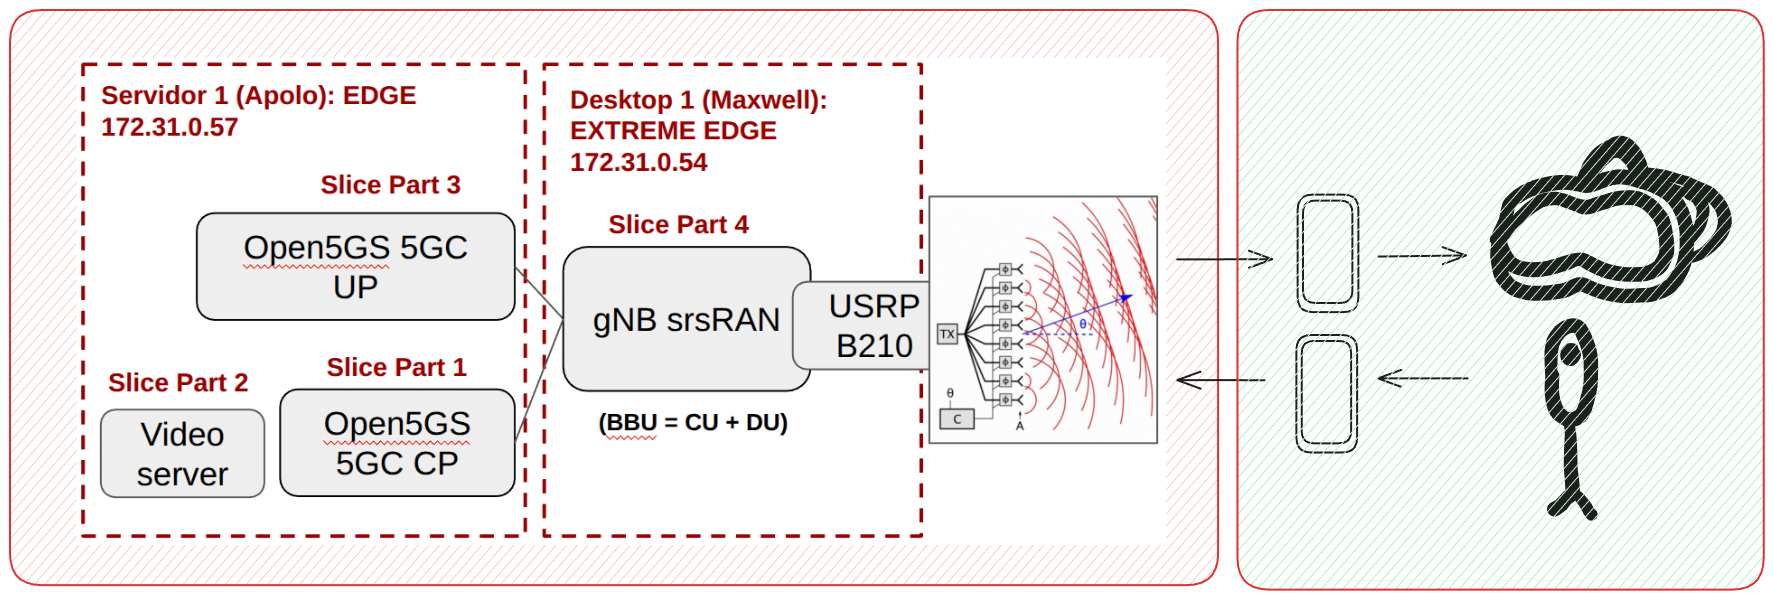
\includegraphics[width=1\linewidth]{etc/simu/obj1.png}
        \caption{Pacote-C e usuários finais.}
    \end{figure}
\end{frame}

\begin{frame}{Desafio Técnico}
    \justifying
    \hspace{0.5cm}O principal desafio técnico no experimento foi identificar 
    protocolos para diminuir o delay final da imagem no óculos vr, além de 
    implementar o servidor utilizando a ferramenta open-source Mediamtx e 
    configura-la para o nosso problema. 
\end{frame}

\begin{frame}{Câmera insta 360 one X}
    \justifying
    \hspace{0.5cm}Para conectar a câmera ao celular, é necessário utilizar o
    aplicativo disponível da empresa insta360 e o protocolo suportado pela
    câmera, RTMP(Real-Time Messaging Protocol). Ao conectar a câmera via wifi, 
    a imagem da câmera é transmitida pelo 5G que será conectada ao pacote C. 
\end{frame}

\begin{frame}
    \begin{columns}
        \column{0.5\textwidth}
        \centering
        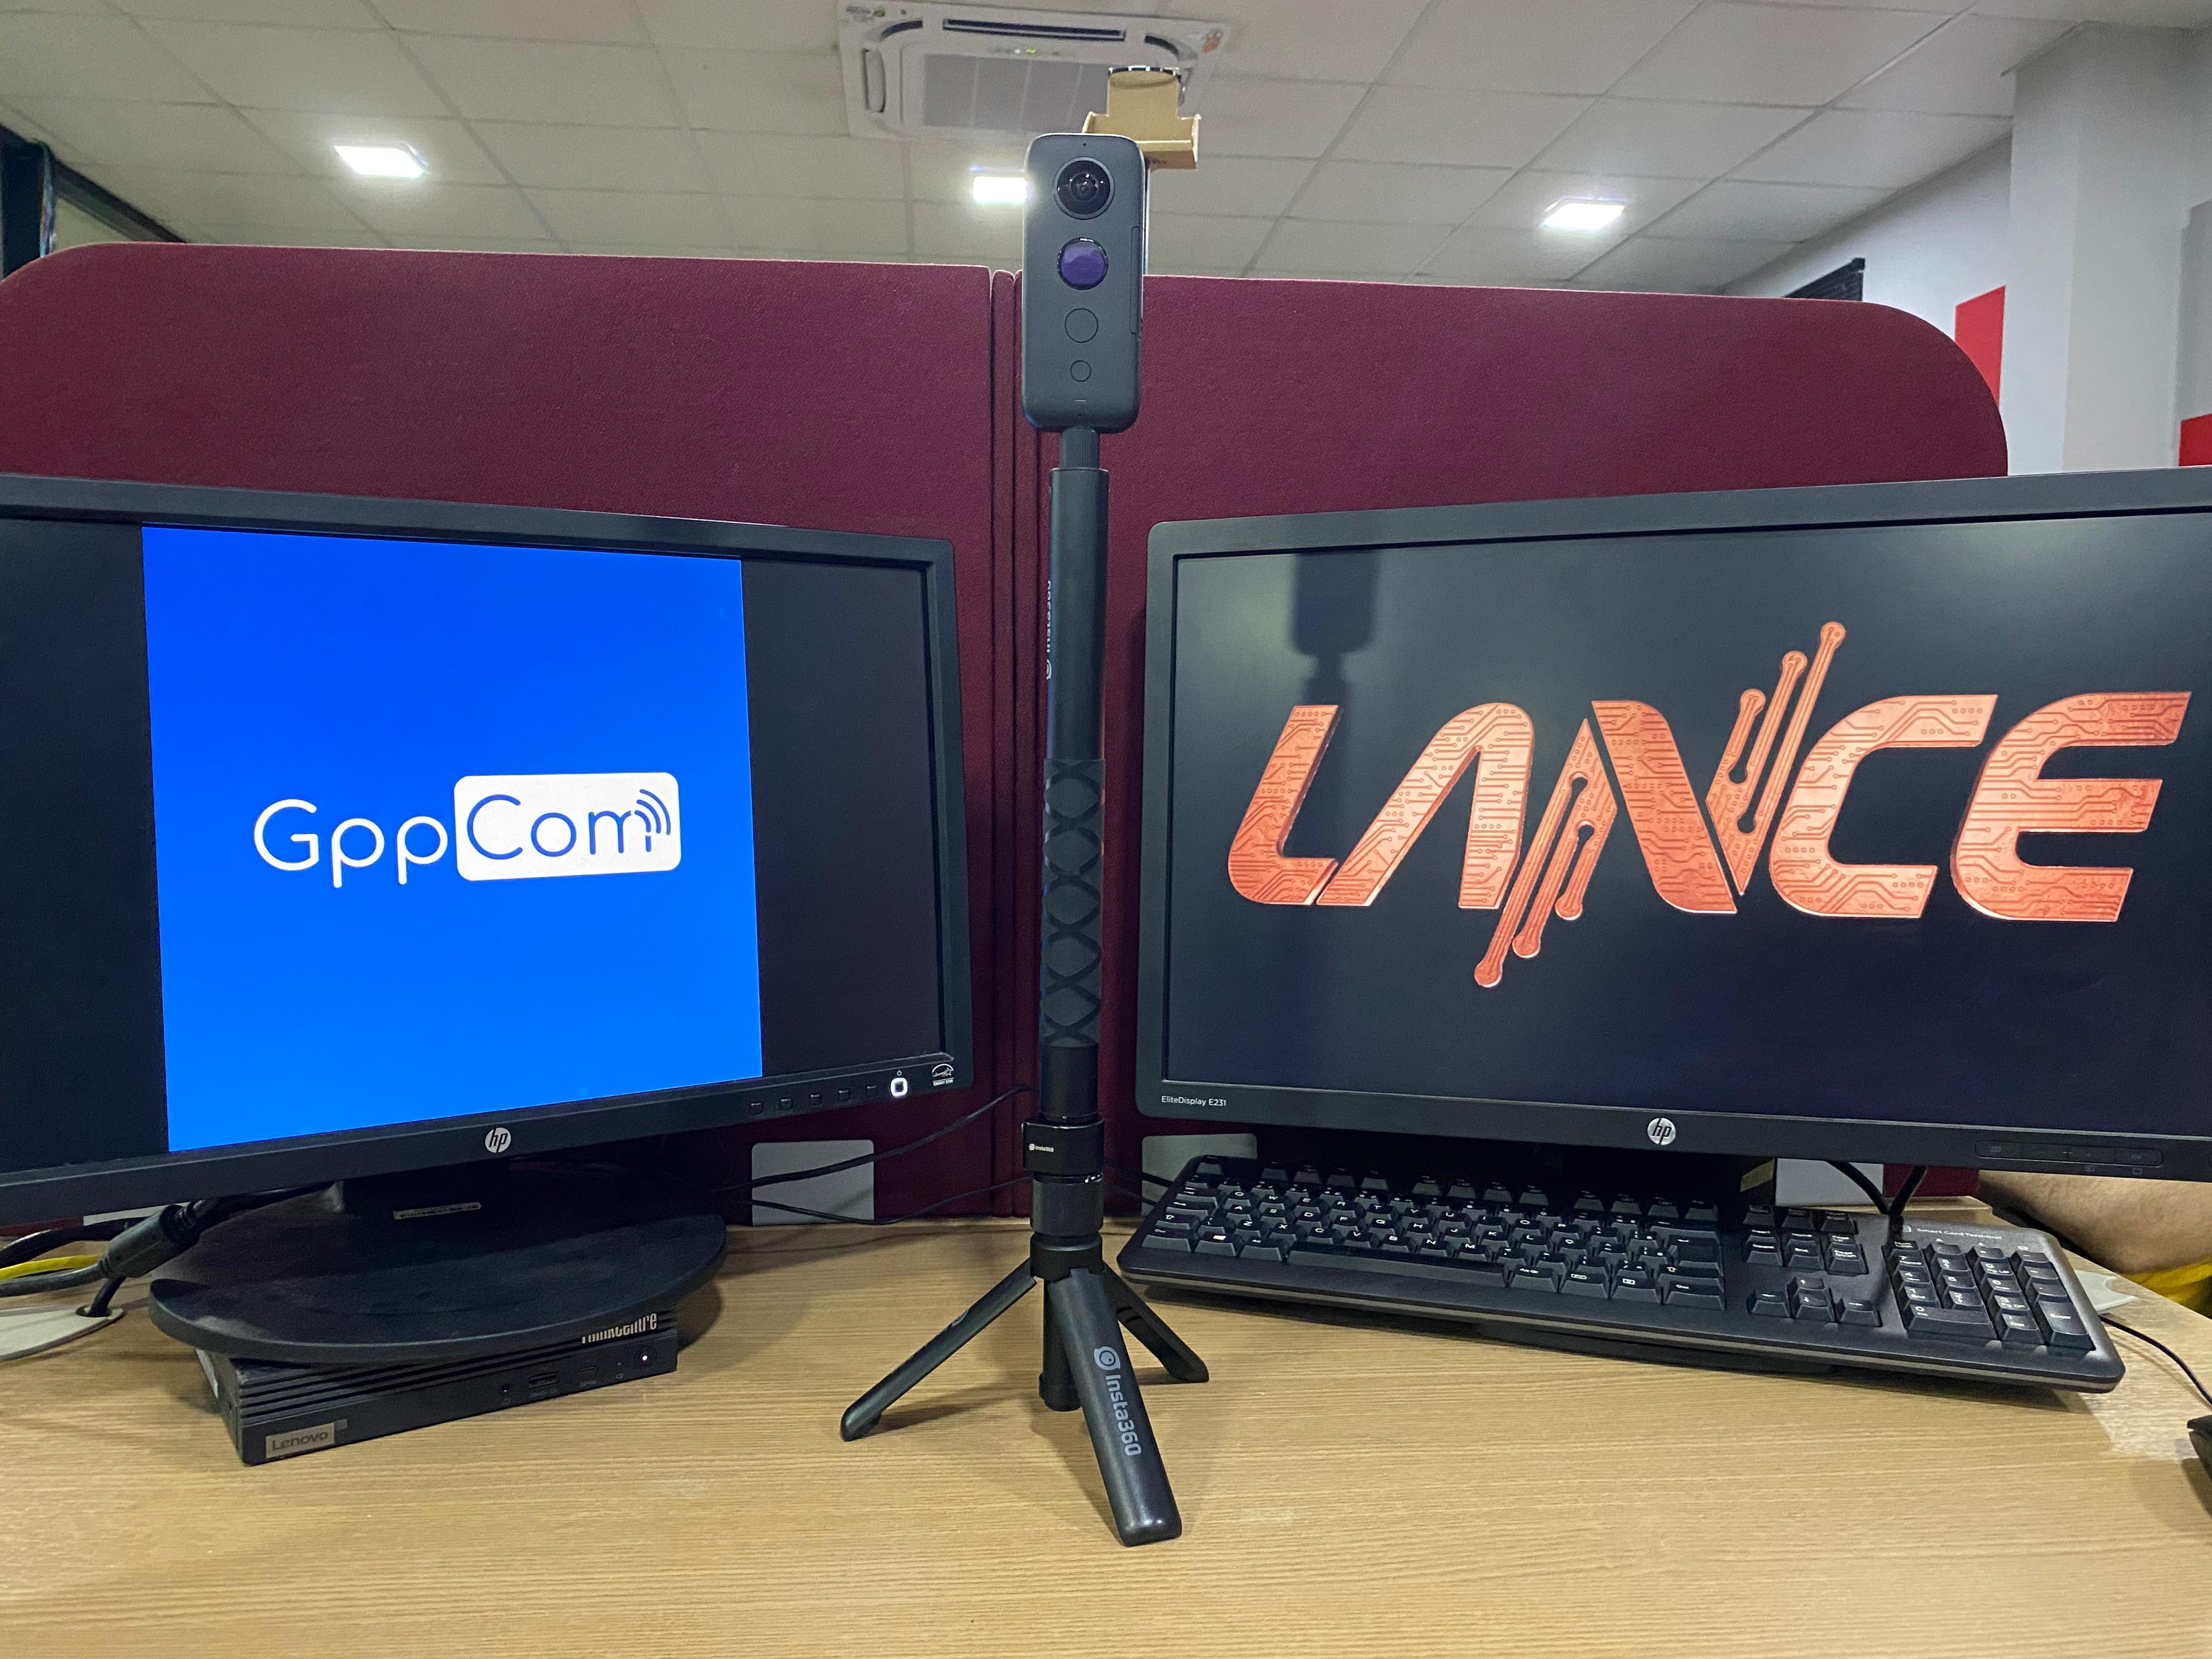
\includegraphics[width=\linewidth]{etc/simu/c1.jpg}

        \column{0.5\textwidth}
        \centering
        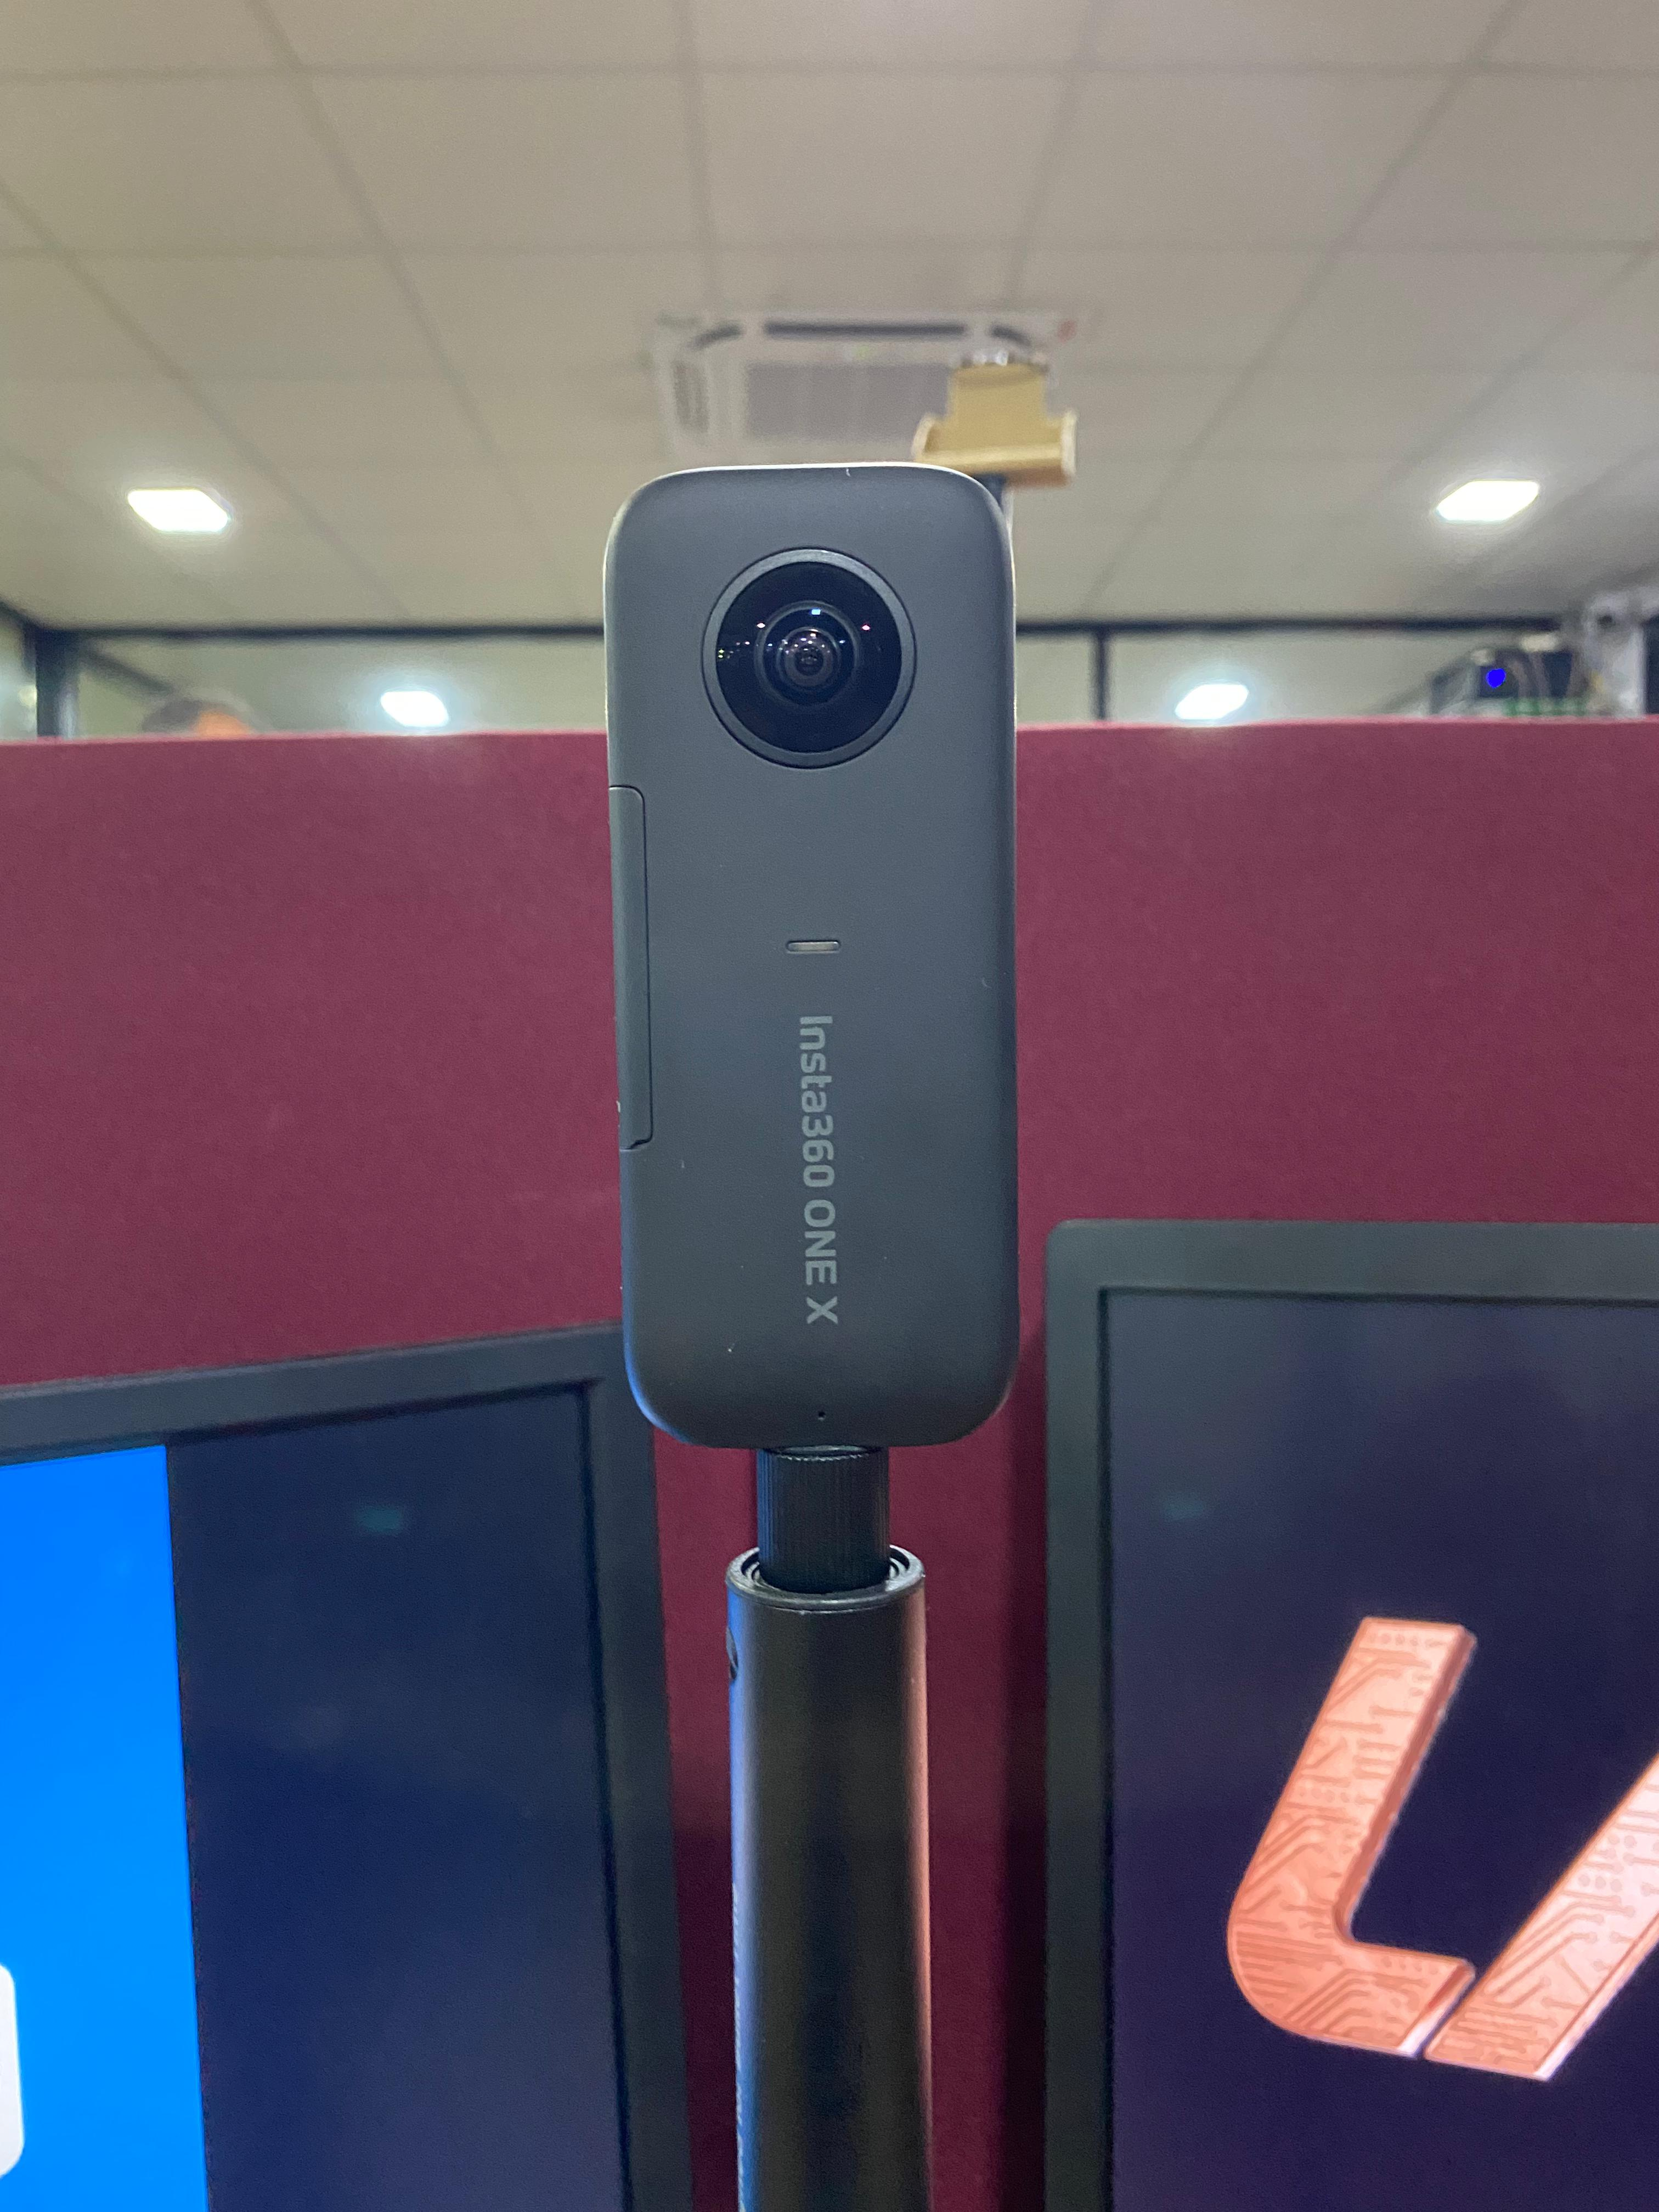
\includegraphics[width=\linewidth]{etc/simu/c2.jpg}
    \end{columns}
\end{frame}

\begin{frame}{Óculos de realidade aumentada MetaQuest3}
    \justifying
    \hspace{0.5cm}O óculos MetaQuest3 pode ser conectado apenas pelo wifi, então
    podemos conectar o óculos a nossa infraestrutura 5G utilizando de técnicas como
    Fixed Wireless Access(FWA) que pode ser disponibilizado por um dos celulares 
    disponíveis no laboratório ou com um dispositivo especifico para FWA como os 
    X doados para o laboratório pela brisanet.
\end{frame}

\begin{frame}
    \begin{columns}
        \column{0.5\textwidth}
        \centering
        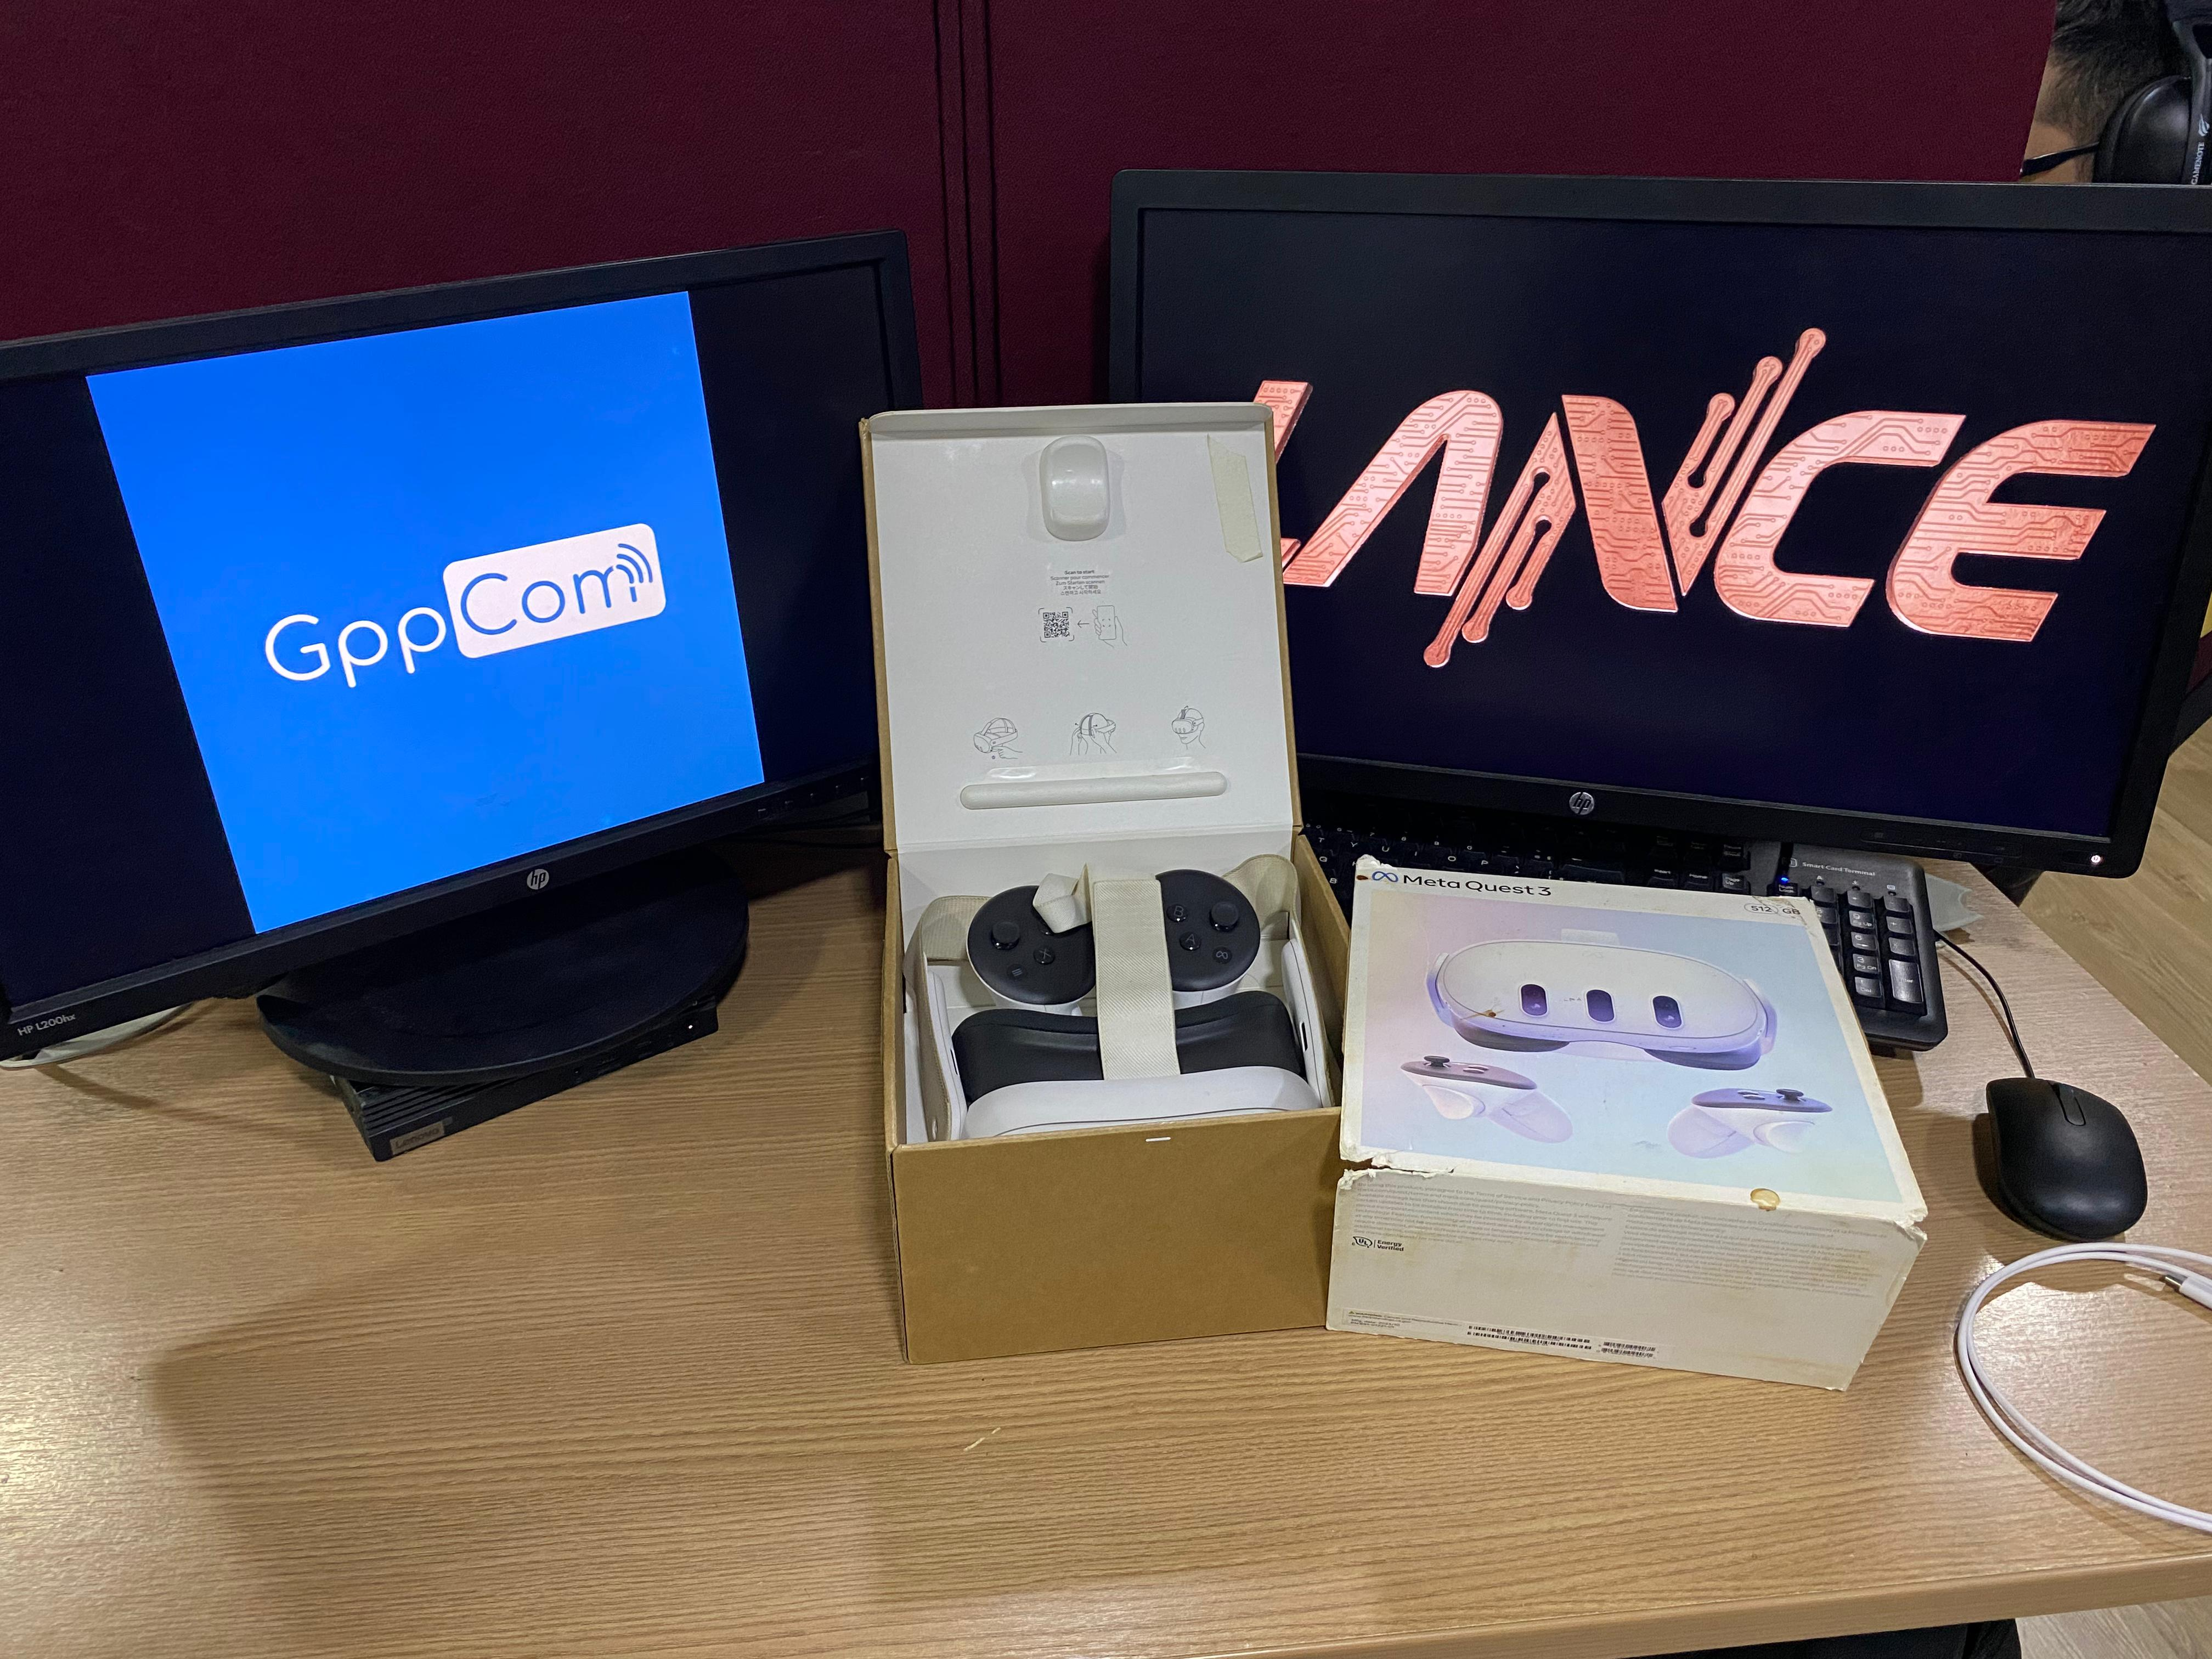
\includegraphics[width=\linewidth]{etc/simu/vr1.jpg}

        \column{0.5\textwidth}
        \centering
        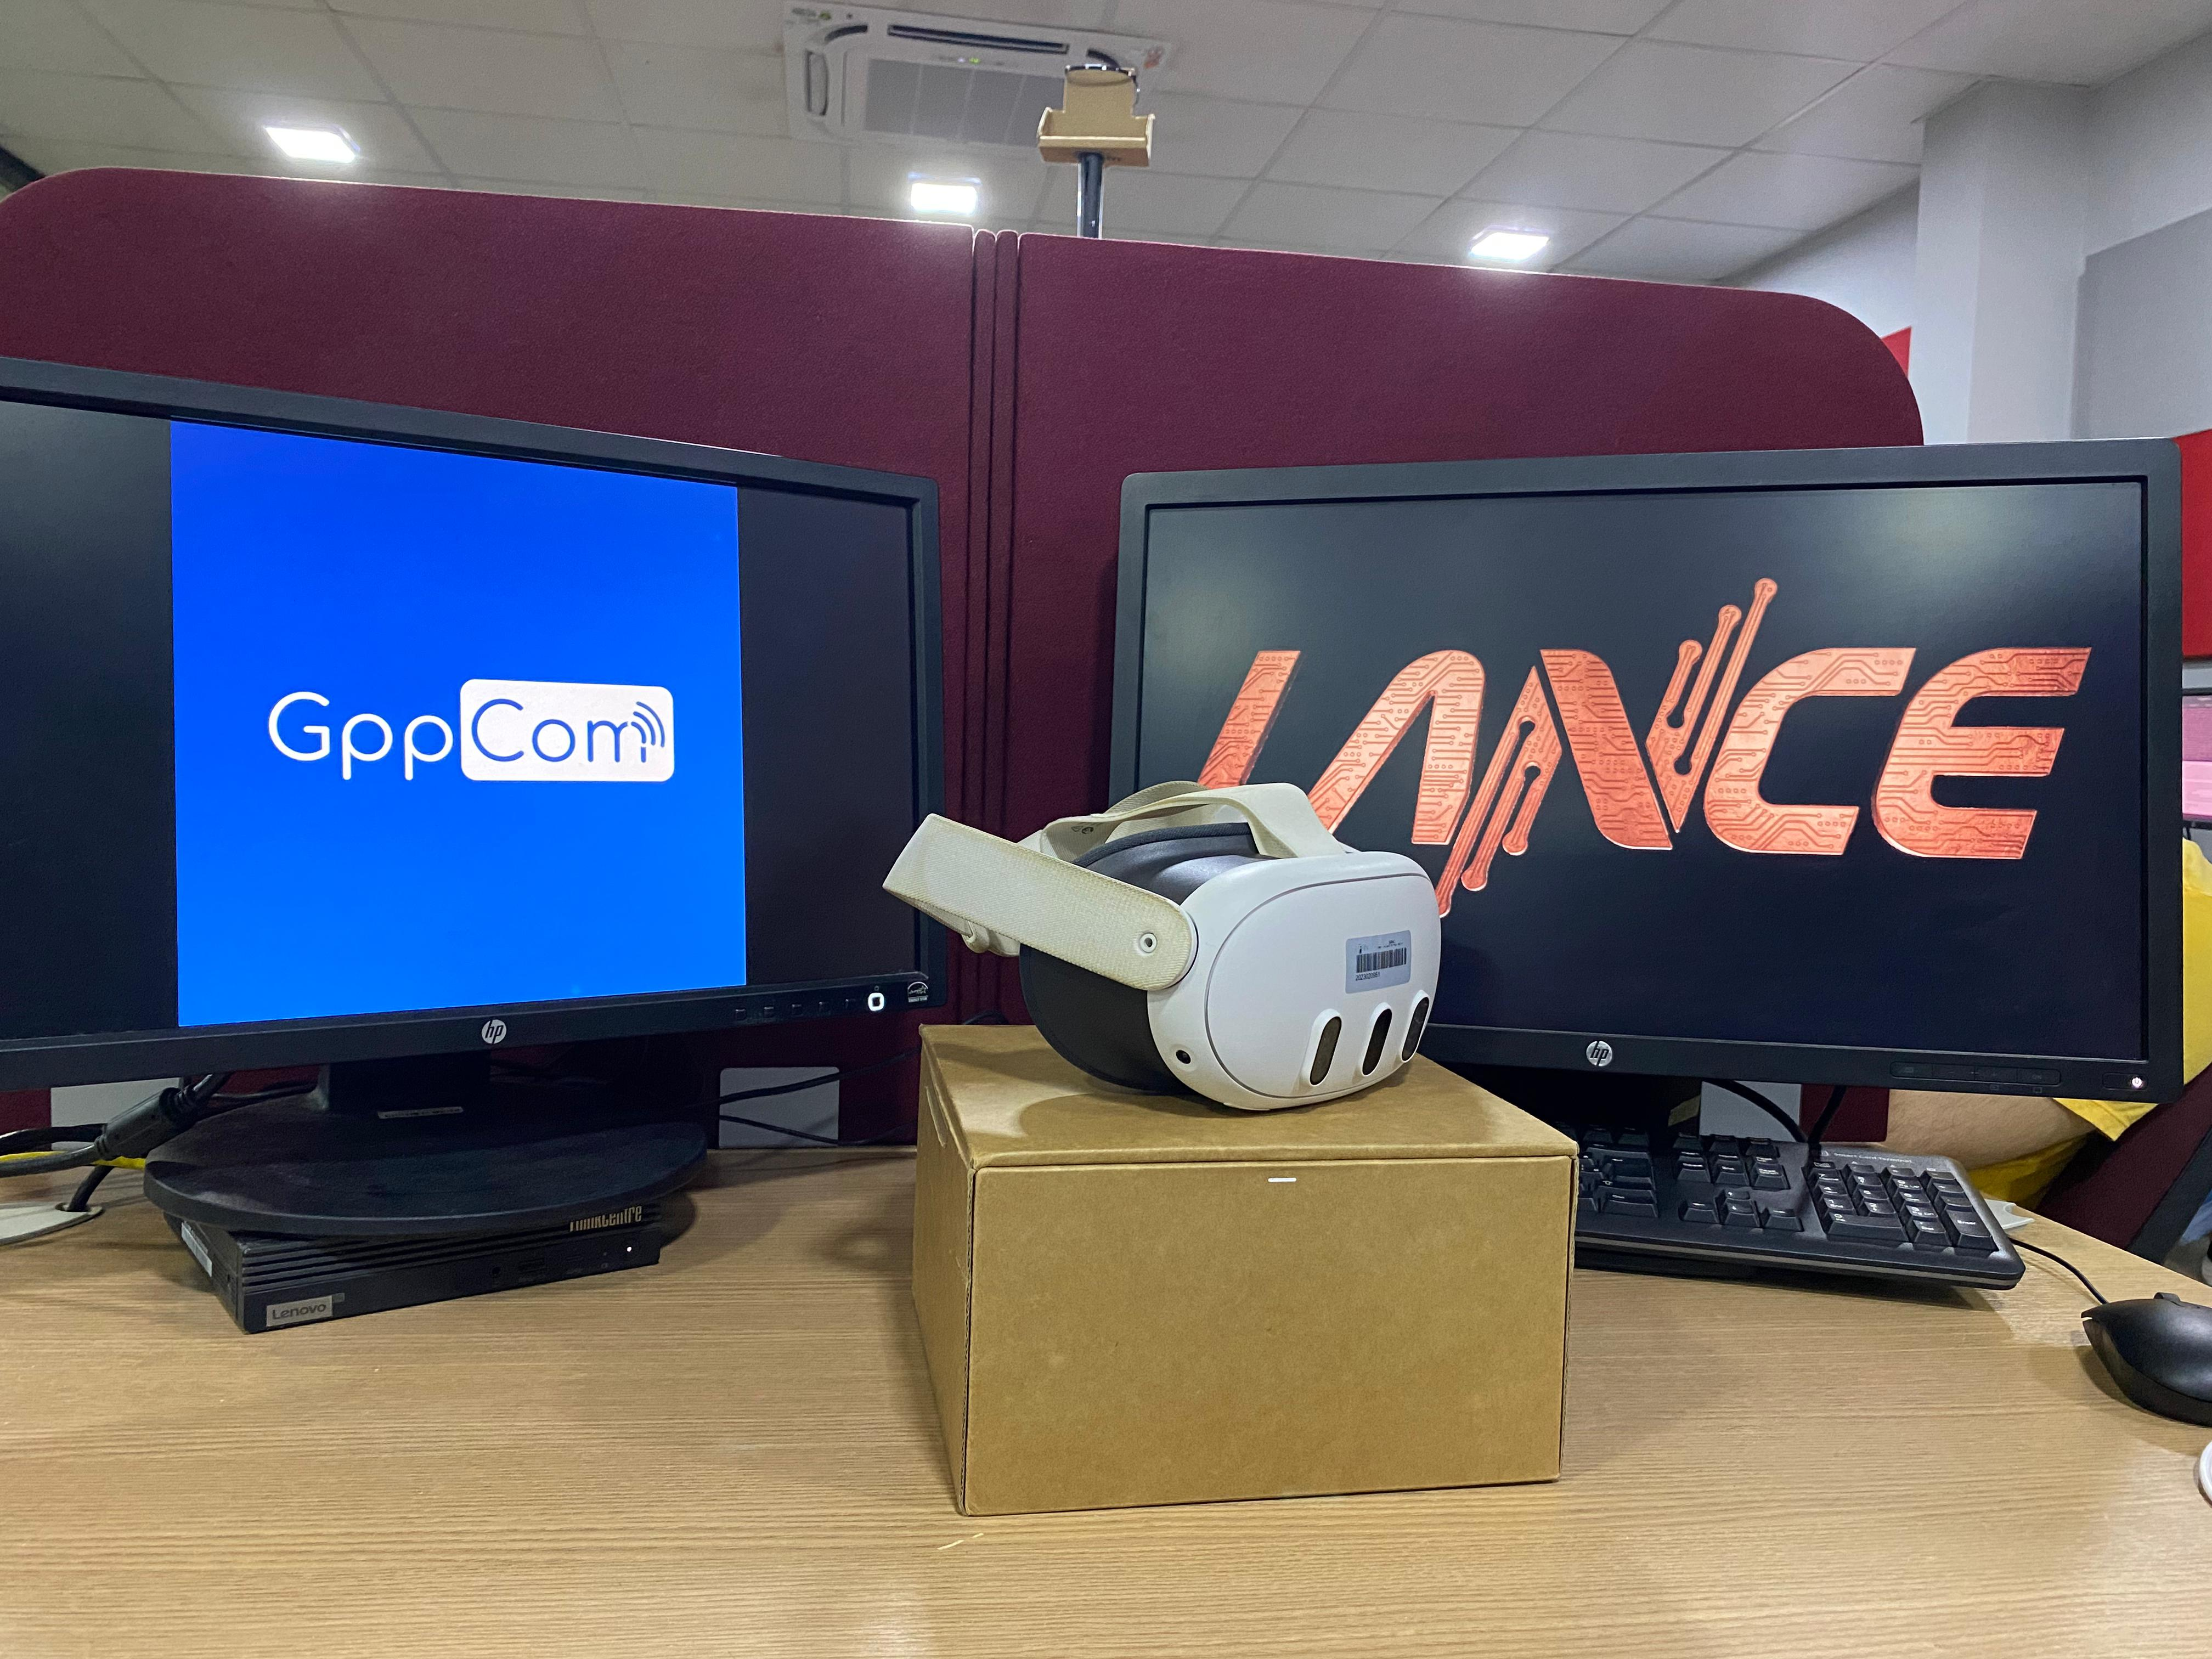
\includegraphics[width=\linewidth]{etc/simu/vr2.jpg}
    \end{columns}
\end{frame}

\begin{frame}
    \begin{columns}
        \column{0.5\textwidth}
        \centering
        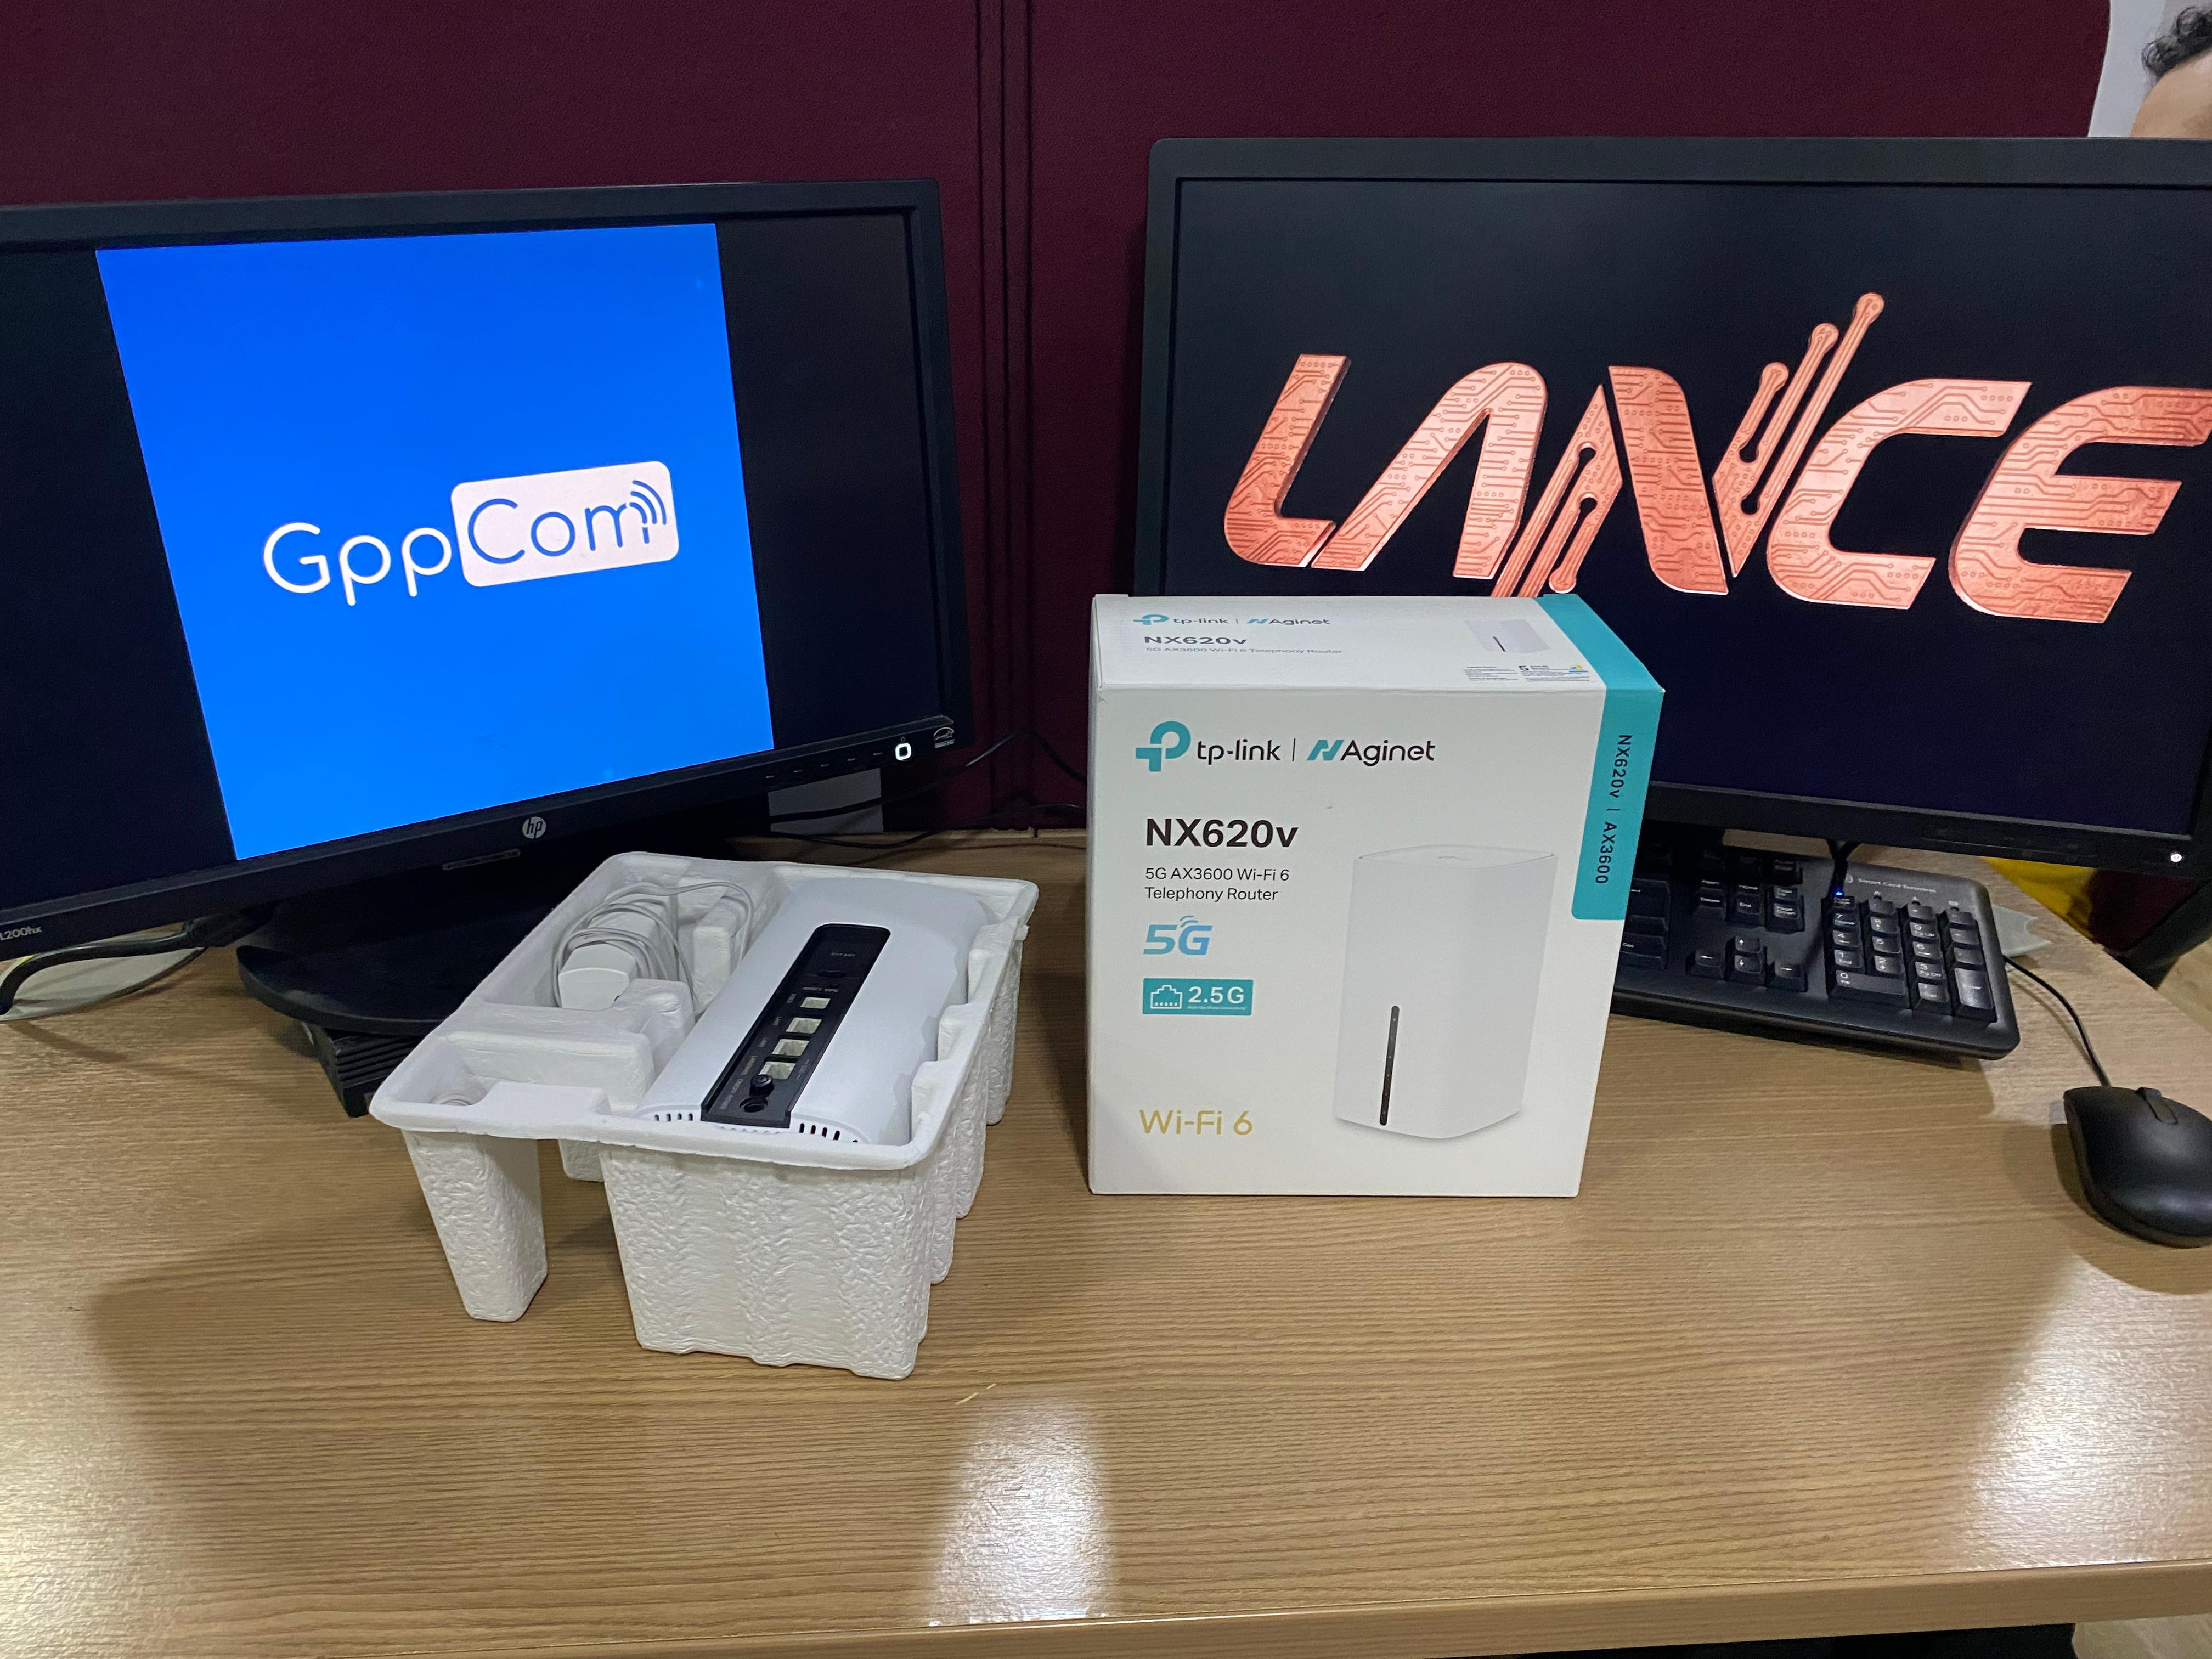
\includegraphics[width=\linewidth]{etc/simu/fwa1.jpg}

        \column{0.5\textwidth}
        \centering
        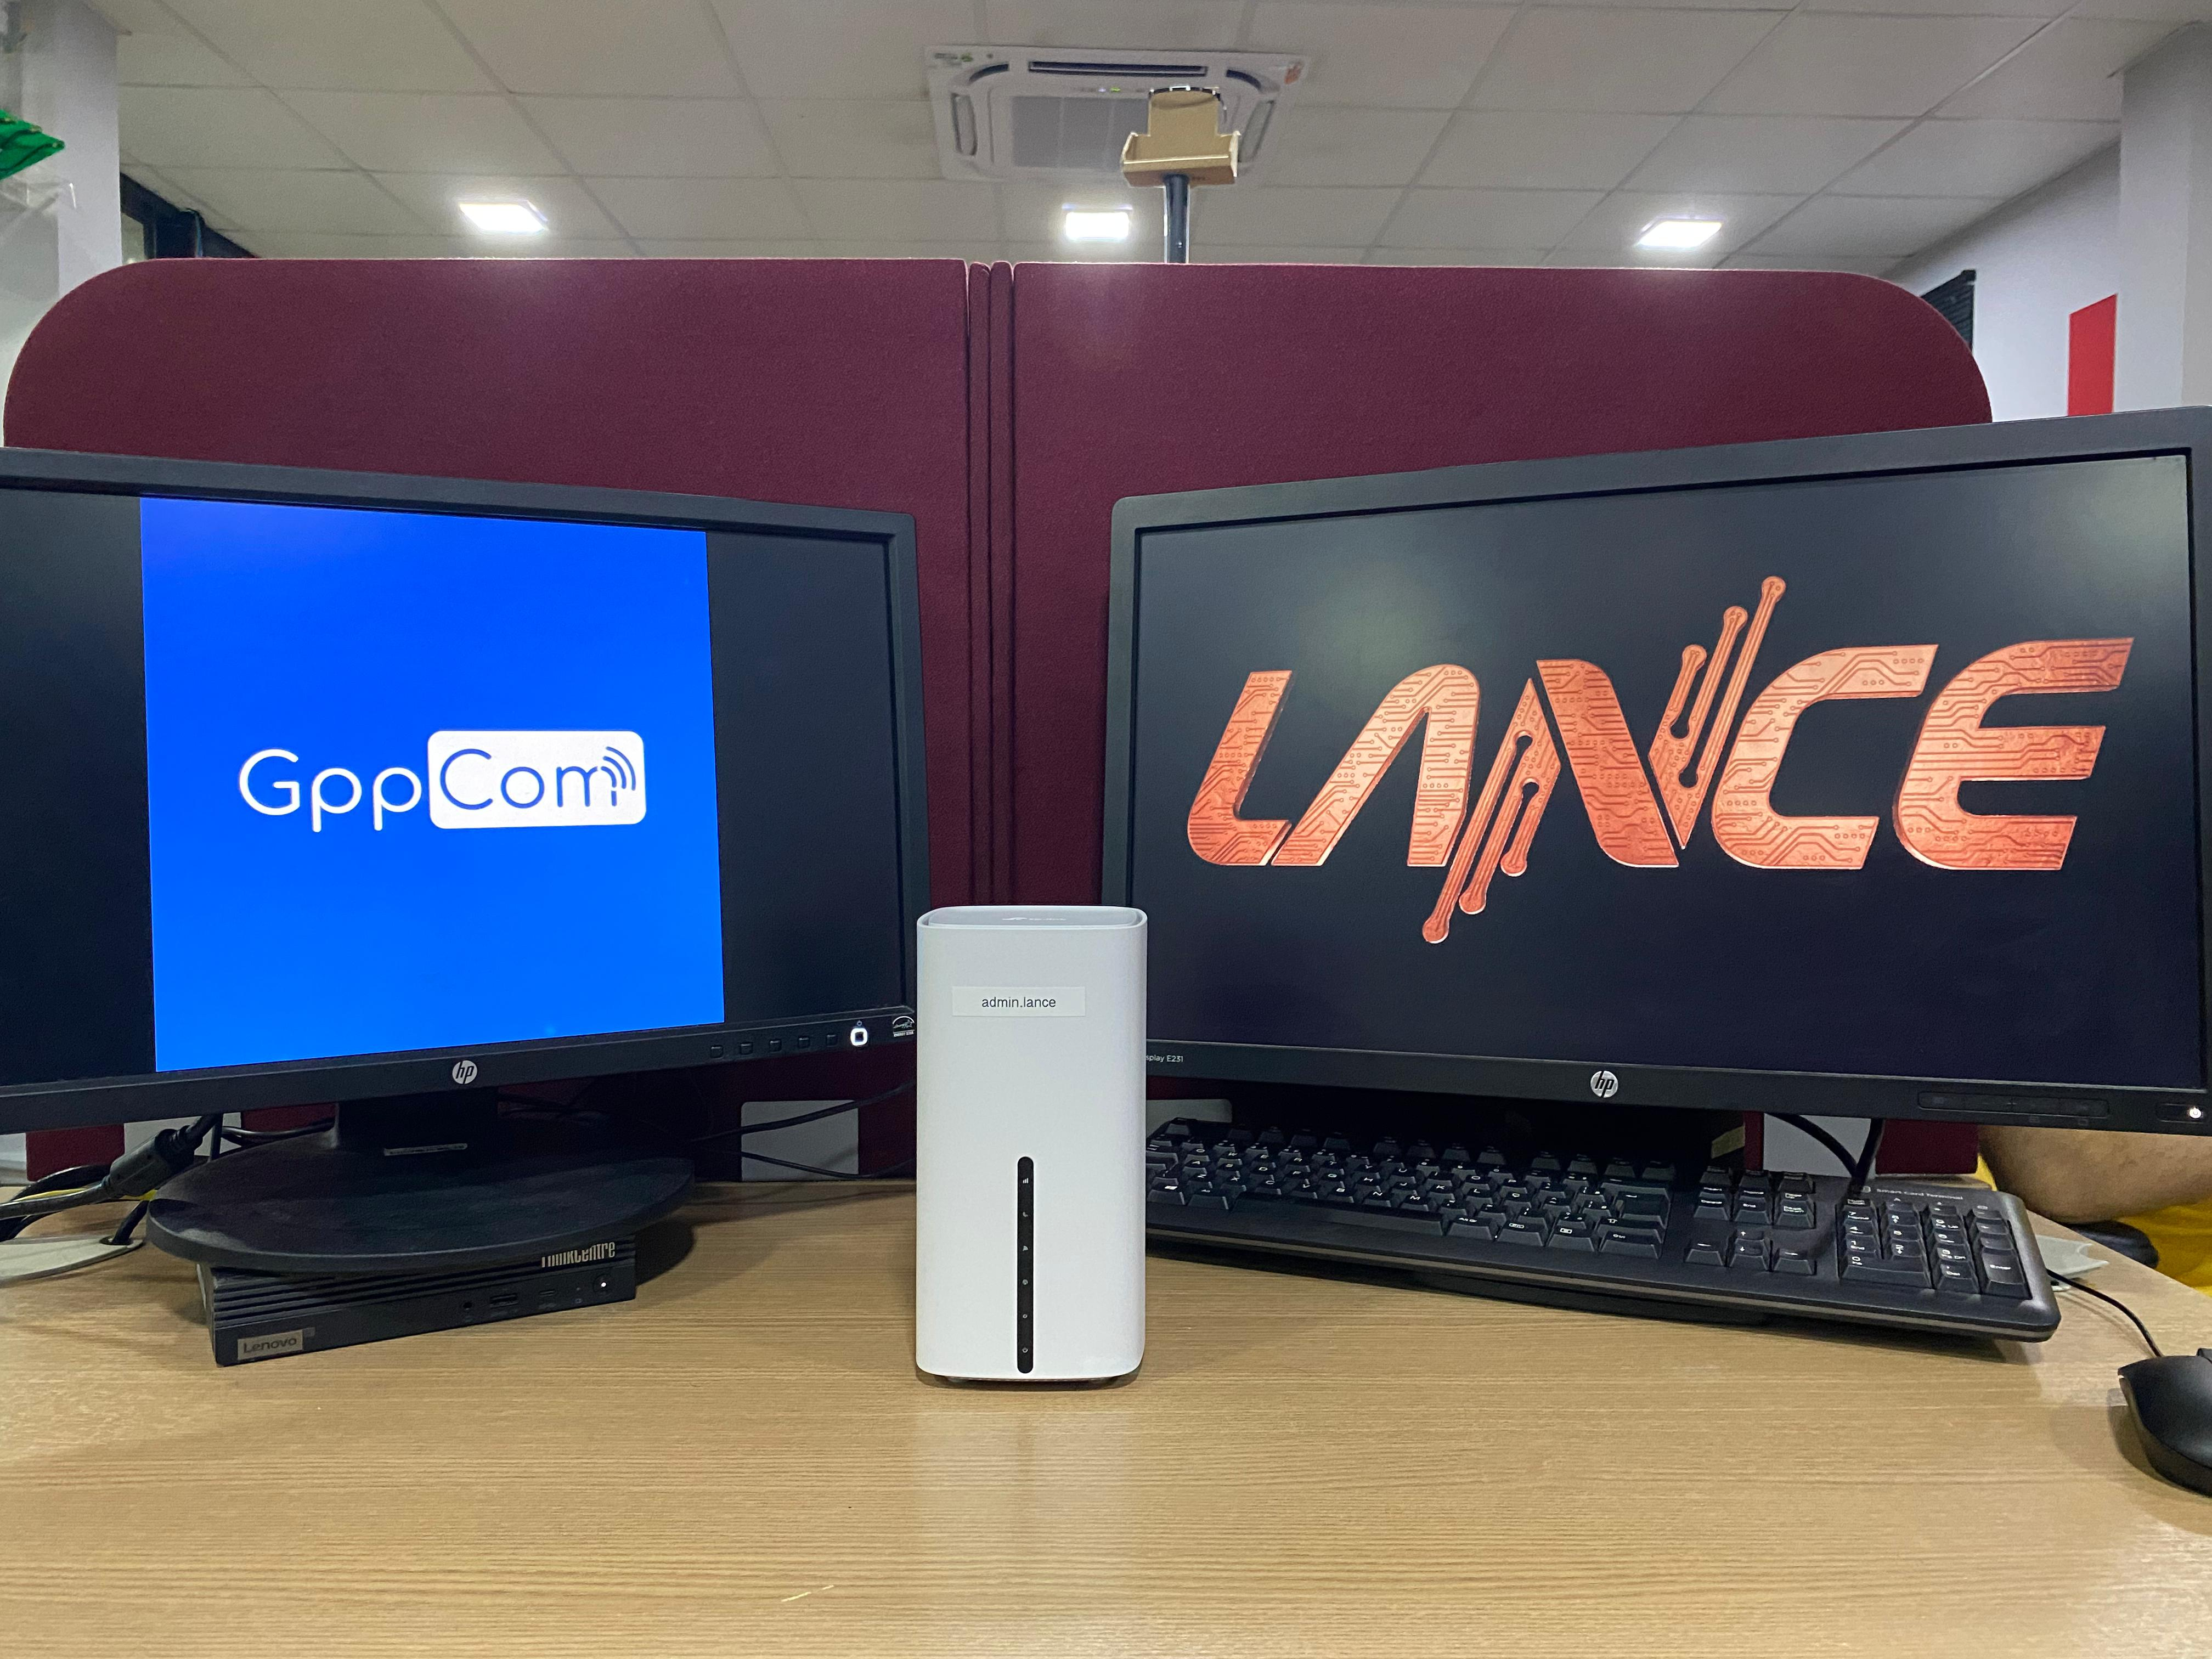
\includegraphics[width=\linewidth]{etc/simu/fwa2.jpg}
    \end{columns}
\end{frame}

\begin{frame}{Solução de Arquitetura}
    \justifying
    \hspace{0.5cm}Agora que podemos conectar tanto o vr quanto a câmera 360 ao 
    pacote C, precisamos criar uma forma de receber as imagens enviadas da câmera 
    e servir ela para os usuários na rede, no nosso caso o vr. Para fazer isso
    foi escolhido a ferramenta open-source Mediamtx com uma imagem do docker para 
    não só receber a transmissão por RTMP mas também para servir com o protocolo 
    webRTC.
\end{frame}

\begin{frame}{Implementação e Configurações}
    \begin{figure}
        \centering
        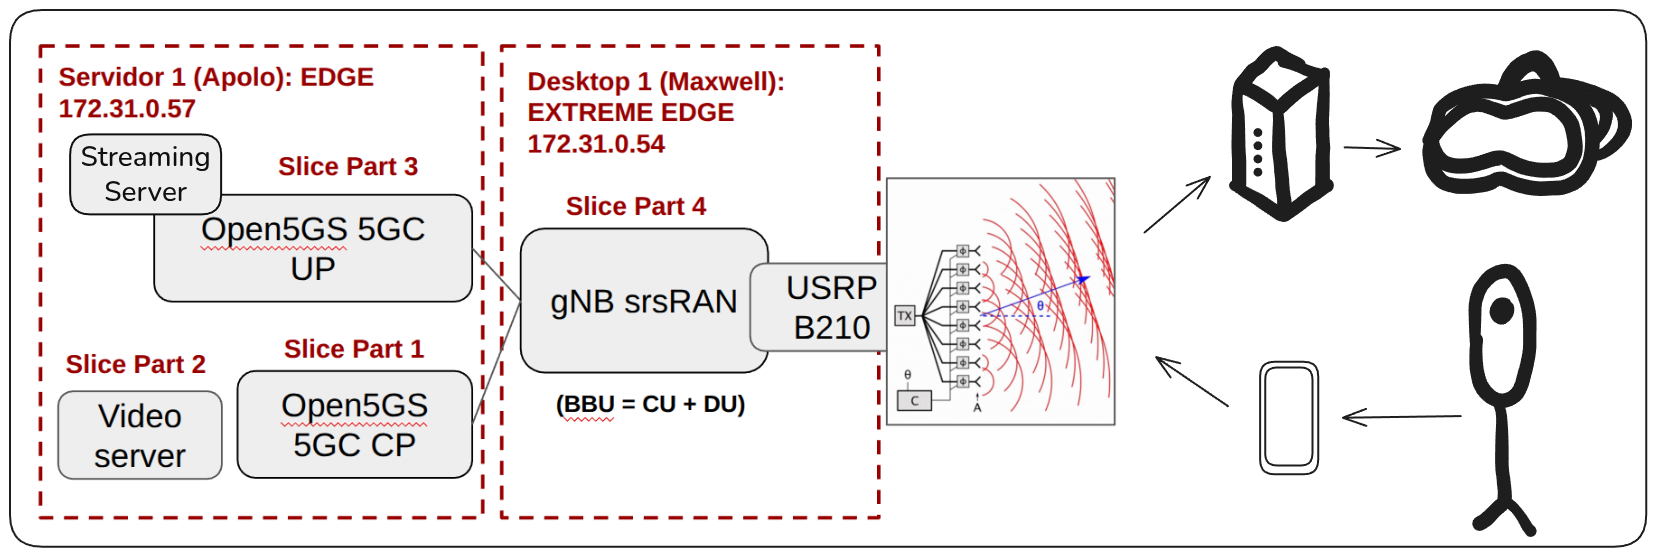
\includegraphics[width=\linewidth]{etc/simu/arquitetura.png}
        \caption{Streaming-Server no Pacote-C}
    \end{figure} 
\end{frame}

%================================================
\section{Resultados}
\begin{frame}{Problemas encontrados}
    \begin{itemize}
        \item Delay de Streaming alto encontrado e limitado pela câmera.
    \end{itemize}
\end{frame}

\begin{frame}
    \begin{figure}
        \centering
        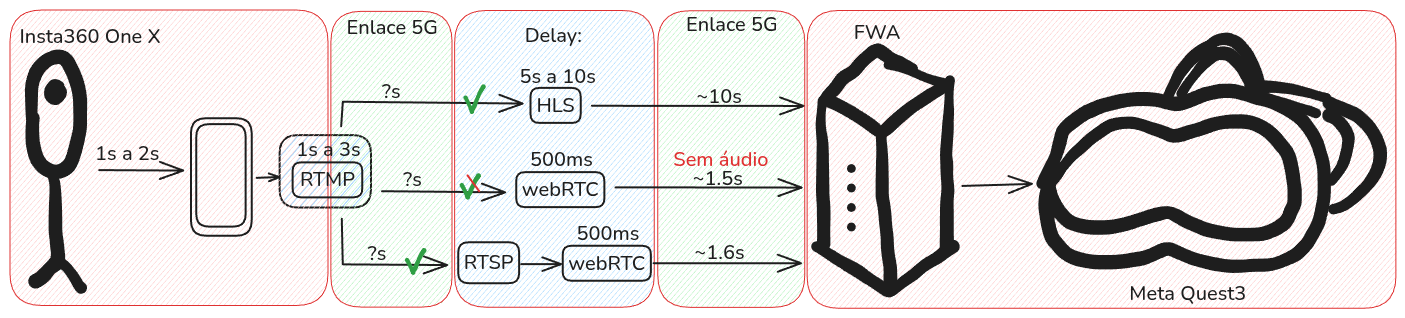
\includegraphics[width=\linewidth]{etc/simu/delay.png}
        \caption{Conexão entre dispositivos de borda e protocolos.}
    \end{figure}
\end{frame}

\begin{frame}{Teste na infraestrutura}
    \justifying
    \hspace{0.5cm}Mostrar o funcionamento
\end{frame}

\begin{frame}
    \begin{figure}
        \centering
        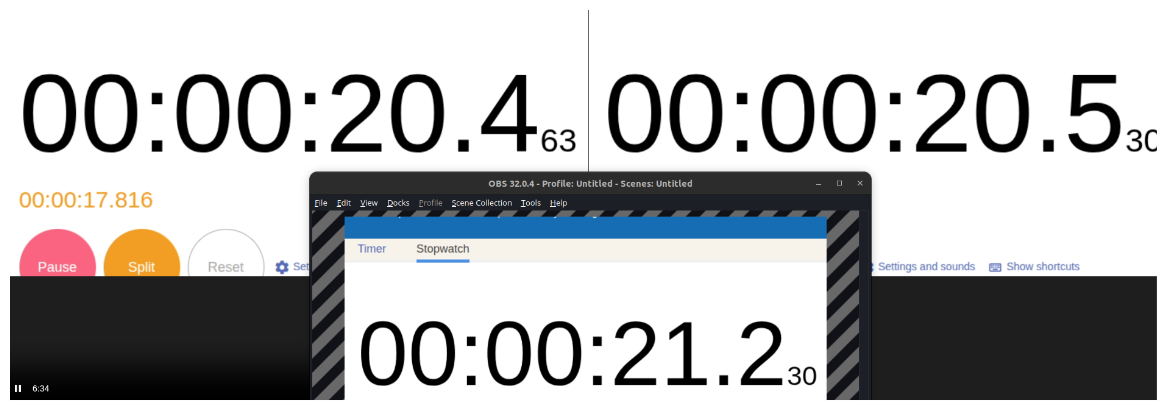
\includegraphics[width=\linewidth]{etc/simu/delayideal.png}
        \caption{Medição inicial de delay ideal}
    \end{figure} 
\end{frame}

\begin{frame}
    \begin{figure}
        \centering
        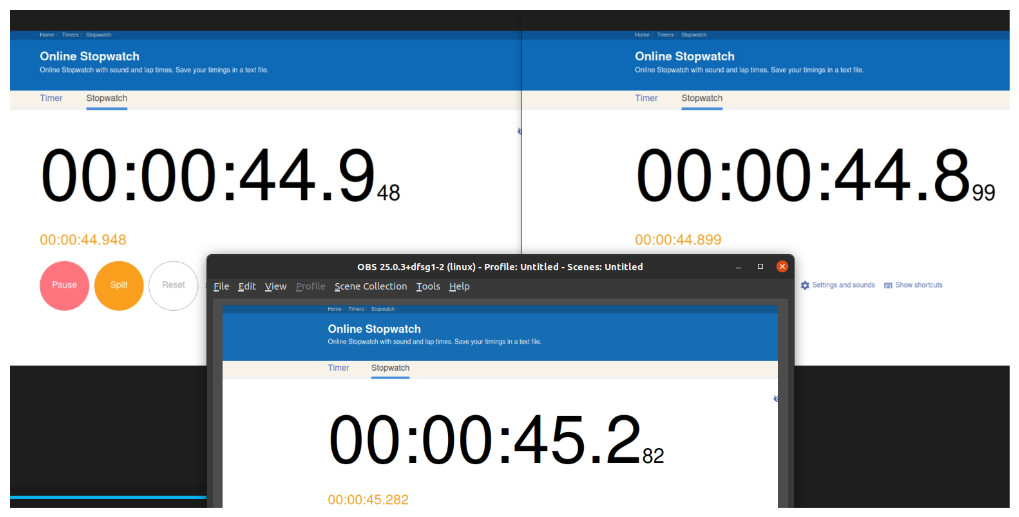
\includegraphics[width=\linewidth]{etc/simu/delay5g.png}
        \caption{Medição inicial de delay 5G}
    \end{figure} 
\end{frame}

\begin{frame}
    \begin{figure}
        \centering
        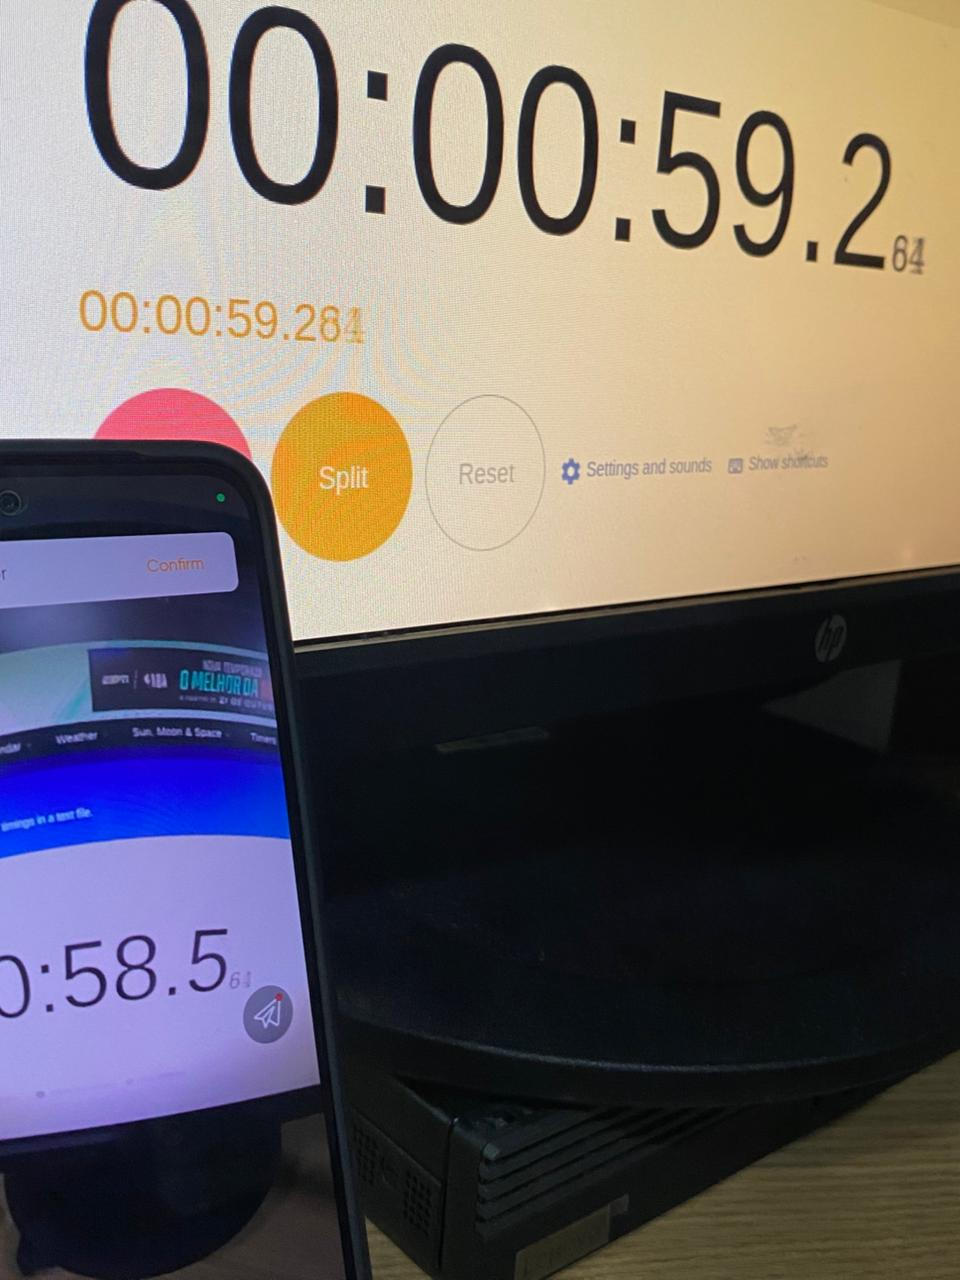
\includegraphics[width=0.45\linewidth]{etc/simu/delayc.jpeg}
        \caption{Medição inicial de delay câmera - celular}
    \end{figure} 
\end{frame}

%================================================
\section{Conclusão}
\begin{frame}{Proximos passos}
    \justifying
    \hspace{0.5cm}Com esse experimento, podemos concluir que novos horizontes de tecnologias
    modernas foram e podem ser adicionadas a infraestrutura do LANCE para novos experimentos 
    em novos paradigmas envolvendo o 5G, como realidade aumentada e Low-latency streaming.
\end{frame}

%================================================
\section{Referências}
%\bibitem{Ex2} citação Disponível em: {\url{link}}. Acesso em: .
\begin{frame}[allowframebreaks]
\small
\begin{thebibliography}{99}
\bibitem{mediamtx}
bluenviron/mediamtx. Disponível em: <{\url{https://github.com/bluenviron/mediamtx}}>. Acesso em: 23 fev. 2026.
\bibitem{overflow}
nginx live streaming too high latency 45 sec. Disponível em: <{\url{https://stackoverflow.com/questions/72323486/nginxlive-streaming-too-high-latency-45-sec}}>. Acesso em: 12 fev. 2026.
\bibitem{stopwatch}
Online Stopwatch - easy to use. Disponível em: <{\url{https://www.timeanddate.com/stopwatch/}}>. Acesso em: 05 mar. 2026.
\end{thebibliography}
\end{frame}

%================================================
\section{Agradecimentos}
\begin{frame}
\centering
O presente trabalho foi realizado com apoio do CNPq, Conselho Nacional de Desenvolvimento Científico e Tecnológico – Brasil
\end{frame}
\end{document}
